%\section{Some Electricity for Data Miners}
\section{A Primer on AC power}
\label{sec:basic}
We will briefly review some background on concepts in AC power
before we describe algorithms for energy disaggregation.

\subsection{Electricity Transmission}
The power we use in our homes and offices is
generated at power plants and transmitted to buildings.
Figure~\ref{fig_powerconnection} illustrates how power
is transmitted and transformed.
%\manishc{Huijuan, did you adapt this figure from another source? (in which
%  case you may want to cite it)}
%\huijuanc{It is drawn by myself.}
Initially, a power plant generates 3-phase electrical power.
The voltage is stepped-up to several hundred kilo-volts for 
transmission.
In power substations, transformers decrease the
voltage. Usually after several substations,
the voltage is decreased to 4,800 volts as medium voltage power.
This medium voltage power is then split for two
different kinds of usage: residential and industrial.
To supply power for industrial or commercial buildings,
a 3-phase transformer changes the voltage to 208 volts or 460 volts.
Finally, a three-wire power service is delivered to end users.
To transmit power to residential buildings,
a 3-phase transformer again steps down the voltage.
The power is then transmitted by power poles, and
a power drum decreases voltage to around 110 volts
in the U.S. or 220 volts in other countries.
In the end, a 2-phase or 3-phase power service
is connected into a home for usage.
\begin{figure}
\centering
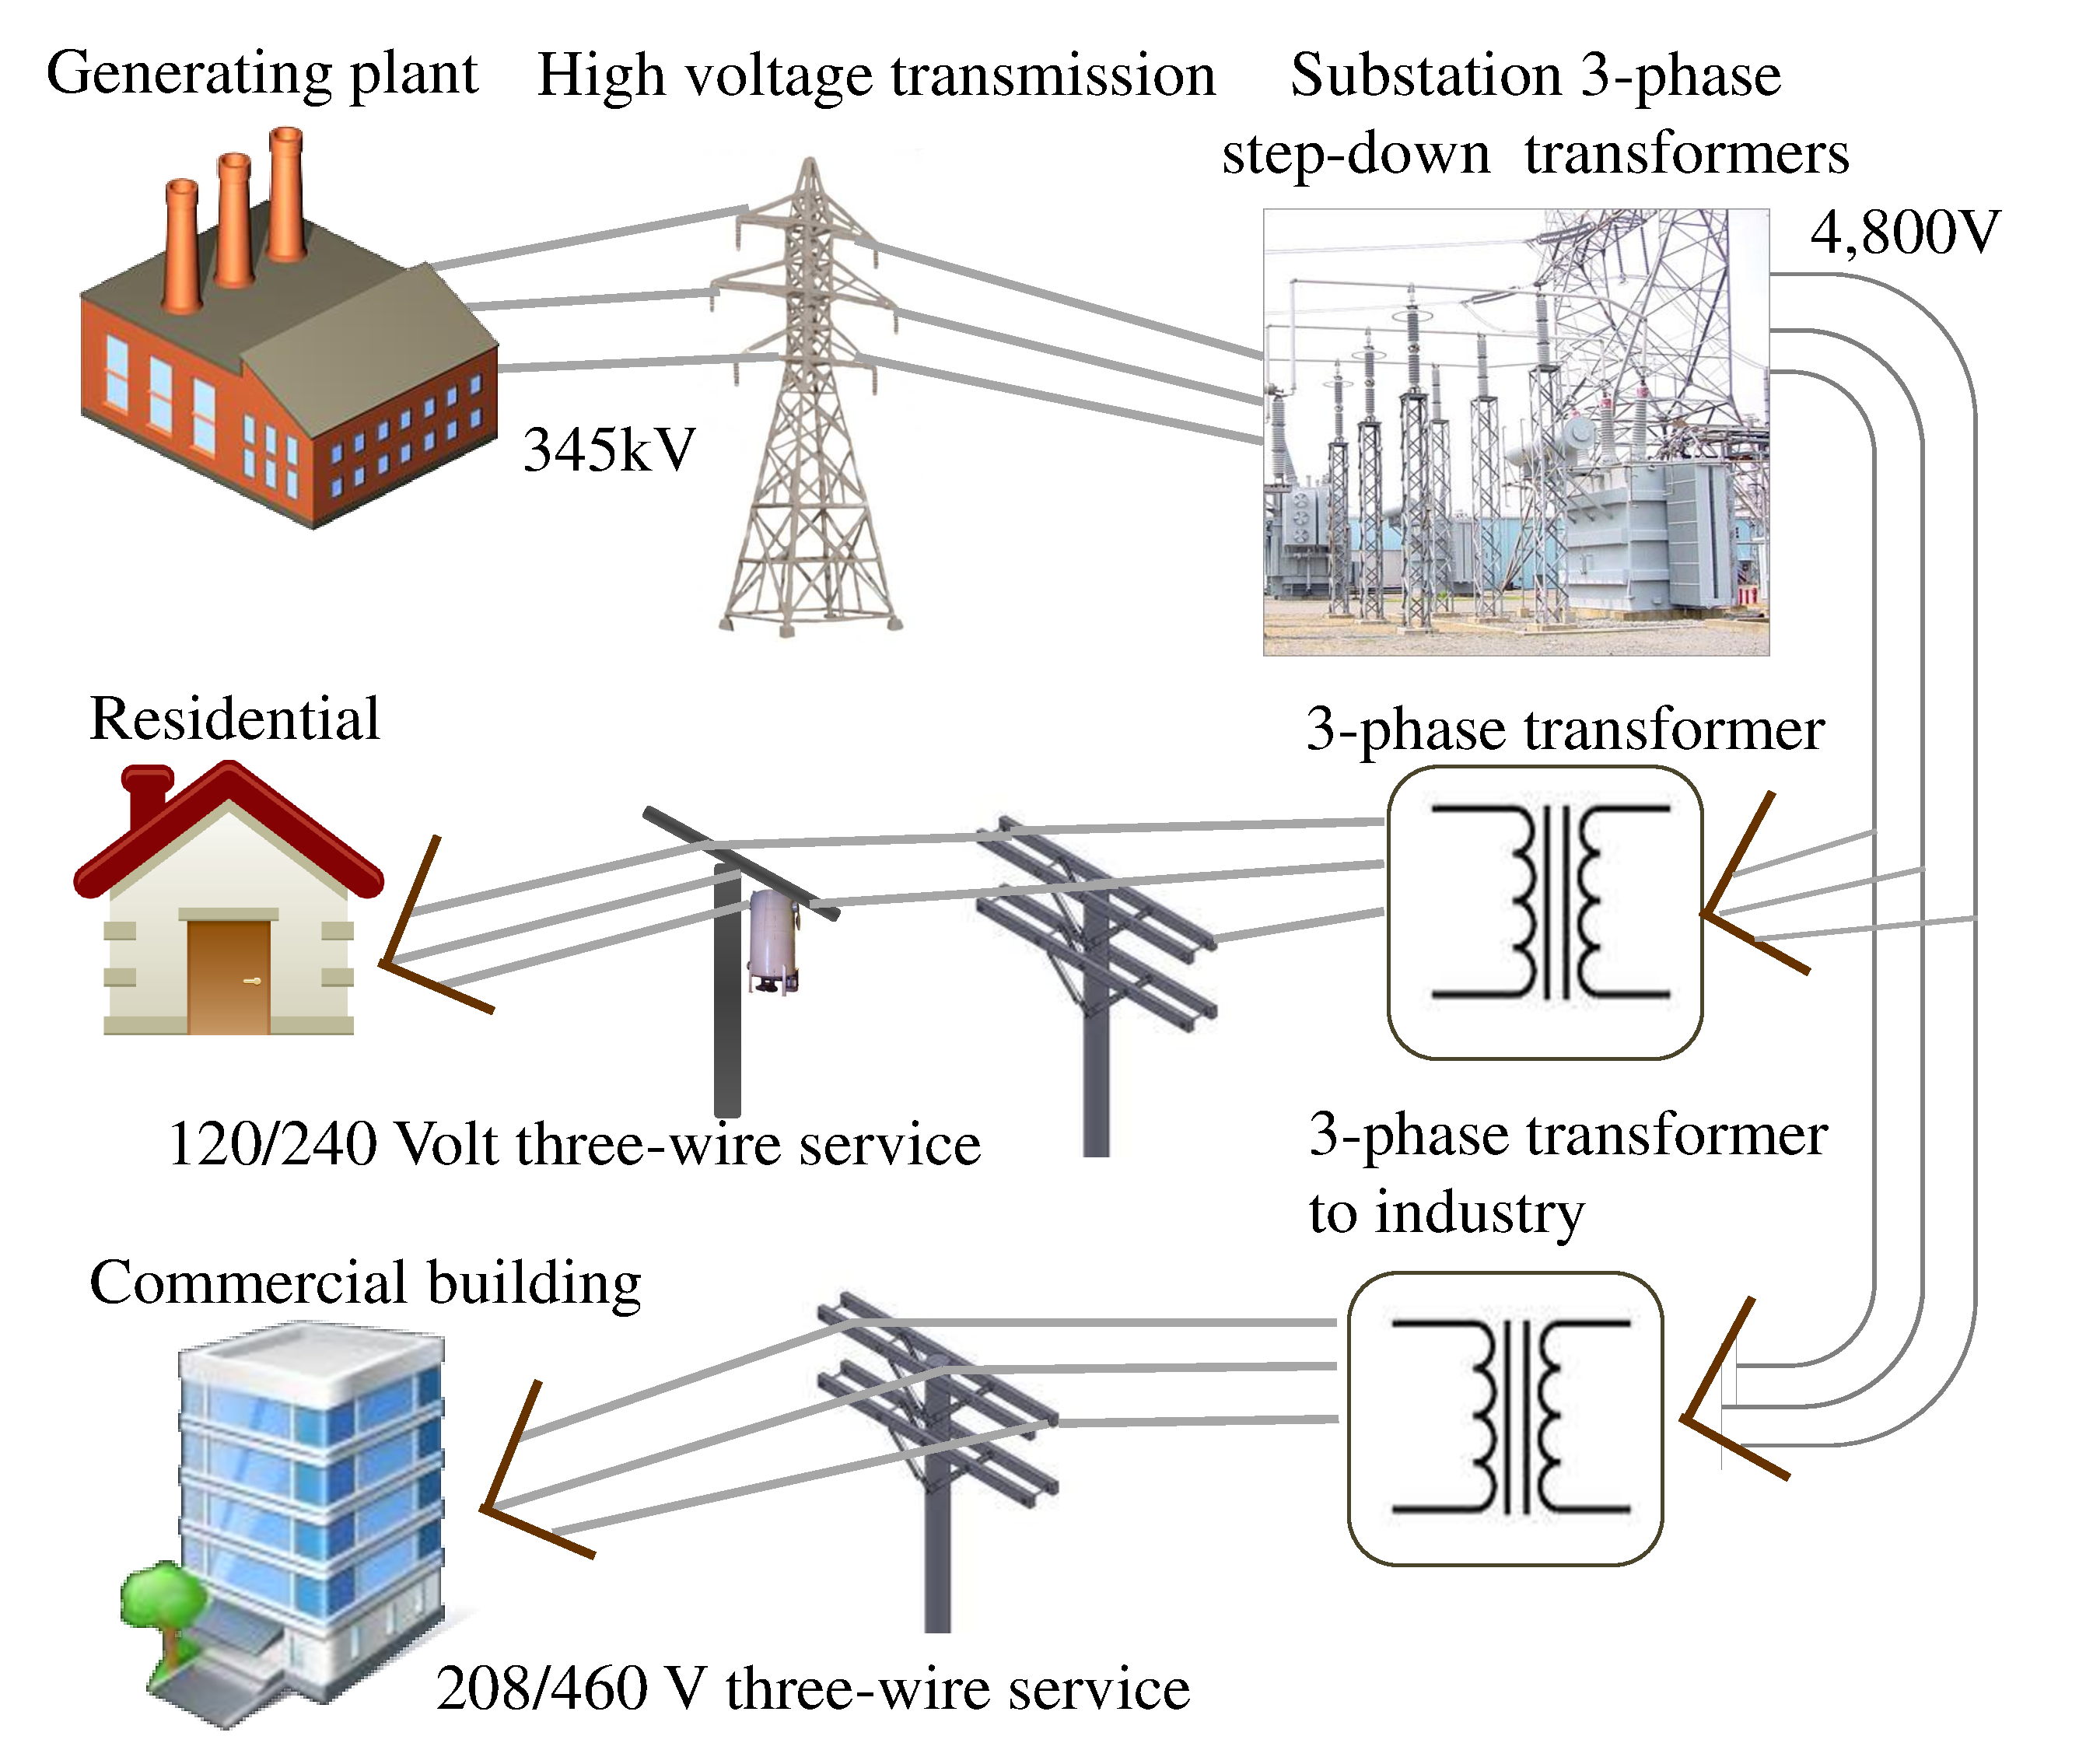
\includegraphics[width=4.5in]{figs/powerConnection.pdf}
\caption{Electricity generation and transmission to residential and commercial buildings.}
\label{fig_powerconnection}
\end{figure}


\subsection{Circuits and Devices}
Normally power in residential or commercial buildings
connects through two or three main phases.
Many circuits then draw power from these main phases
in parallel or in series.
\begin{figure*}[h]
	\centering{
    \begin{tabular}{cc}	
	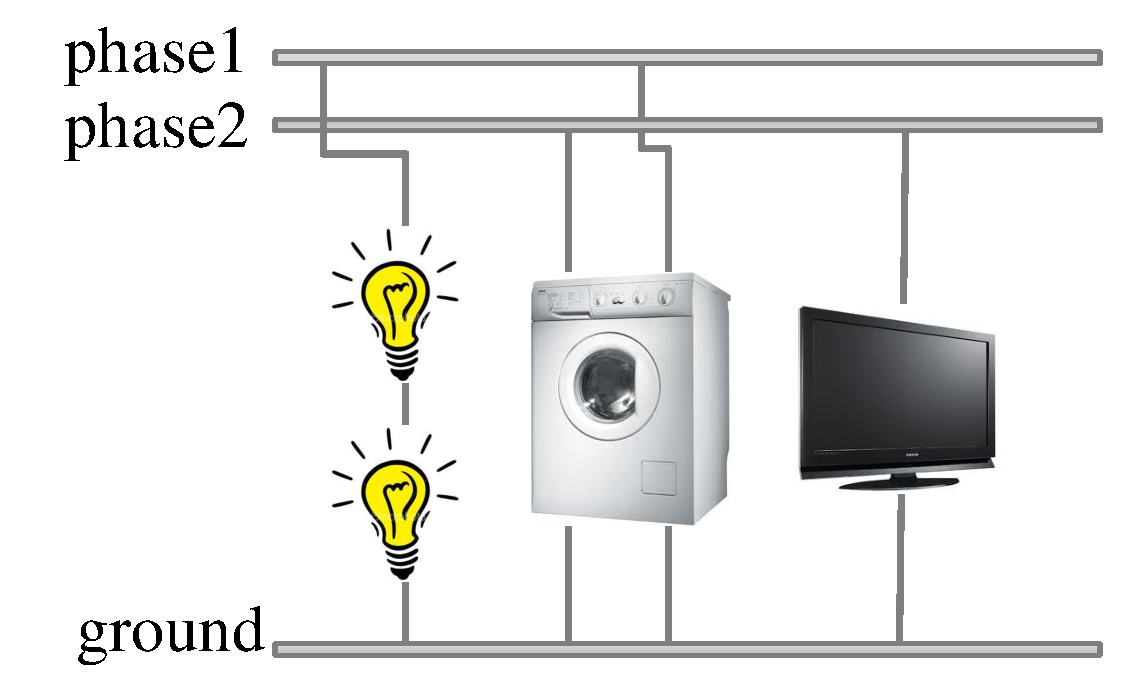
\includegraphics[width=0.43\textwidth]{figs/residentialBG.pdf} \hspace{1em}&
	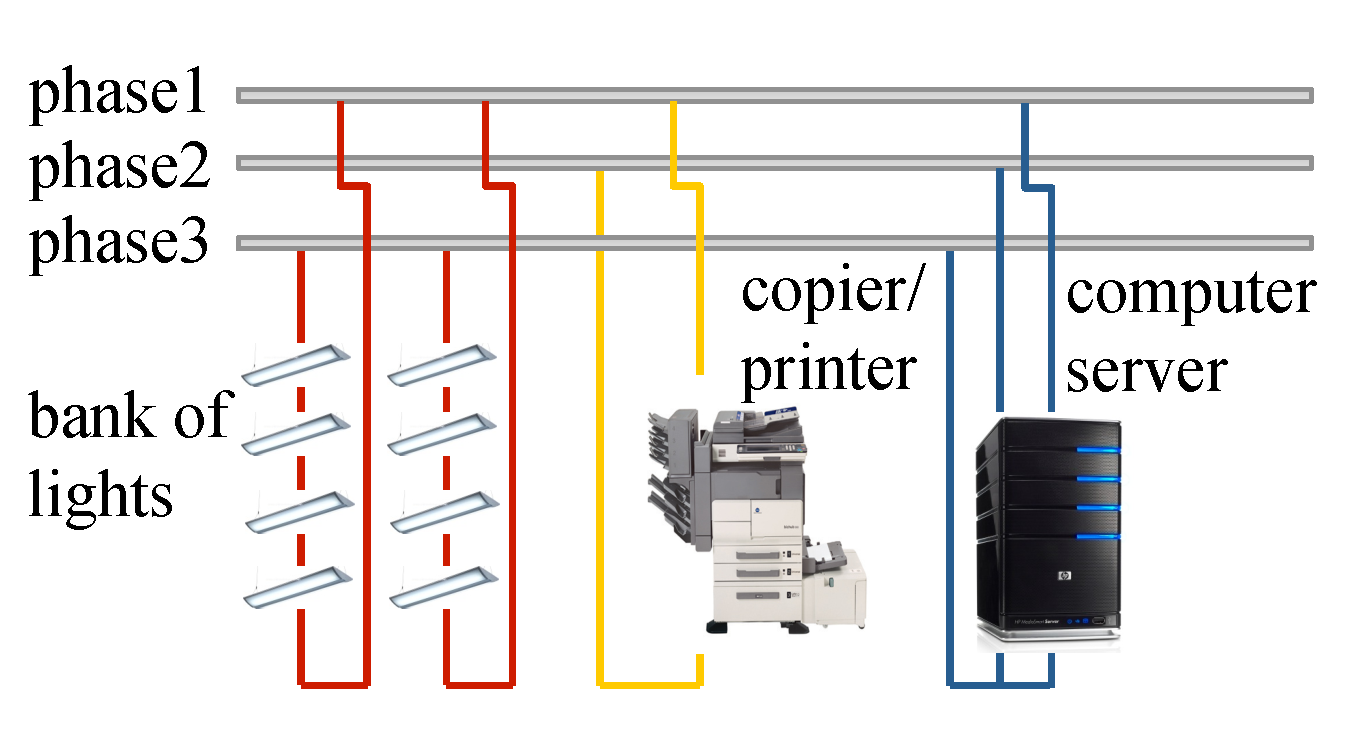
\includegraphics[width=0.5\textwidth]{figs/commercialBG.pdf}\tabularnewline
    (a) & (b) \tabularnewline
    \end{tabular}
    }
	\caption{Example of a circuit in (a) residential building and (b) commercial building.}
    \label{fig_residentialCommercialBG}
\end{figure*}

While most residential devices connect to a single phase some
heavy duty appliances require a two-phase connection.
Figure~\ref{fig_residentialCommercialBG} (a) depicts a typical connection
in residential buildings. 
There are two main phases: phase1 and phase2.
Three circuits connect into these two phases.
In the first circuit, two lights connect in series to phase 1 and the ground.
In the second circuit, a washer/dryer connects to both phases.
In the third circuit, a television connects to phase2 and the ground.
Note that it is possible that several devices
connect to one phase in a circuit.

An example of
a circuit in a commercial building is
depicted in Figure~\ref{fig_residentialCommercialBG} (b).
Devices in any circuit connect to two or all of 
the three phases. 
%\manishc{what about three-phase load?}
%\huijuanc{update this figure: computer server connects to three phases.}
There are two circuits connecting to phase1 and phase3 in red.
Both these circuits supply power to a bank of lights.
Therefore, when people switch on/off,
these lights powers on/off at the same time.
A copier/printer draws power from phase1 and phase2 in yellow. 
A computer server connects to all three phases in blue.

\subsection{Voltage and Current}
%After 3-phase or 2-phase voltage
%is made available to a building and 
%devices connect through these phases, 
%the power connection is effective for the building.
The voltage transmitted from
a power plant is typically 3-phase sinusoidal.
Figure~\ref{fig_threephase} depicts the
waveform of the three phases of AC power.
Each phase $V_1$, $V_2$, $V_3$ has a sinusoidal
voltage waveform. Between each phase,
there's a phase angle difference of $\pi/3$.
\begin{figure}[h]
\centering
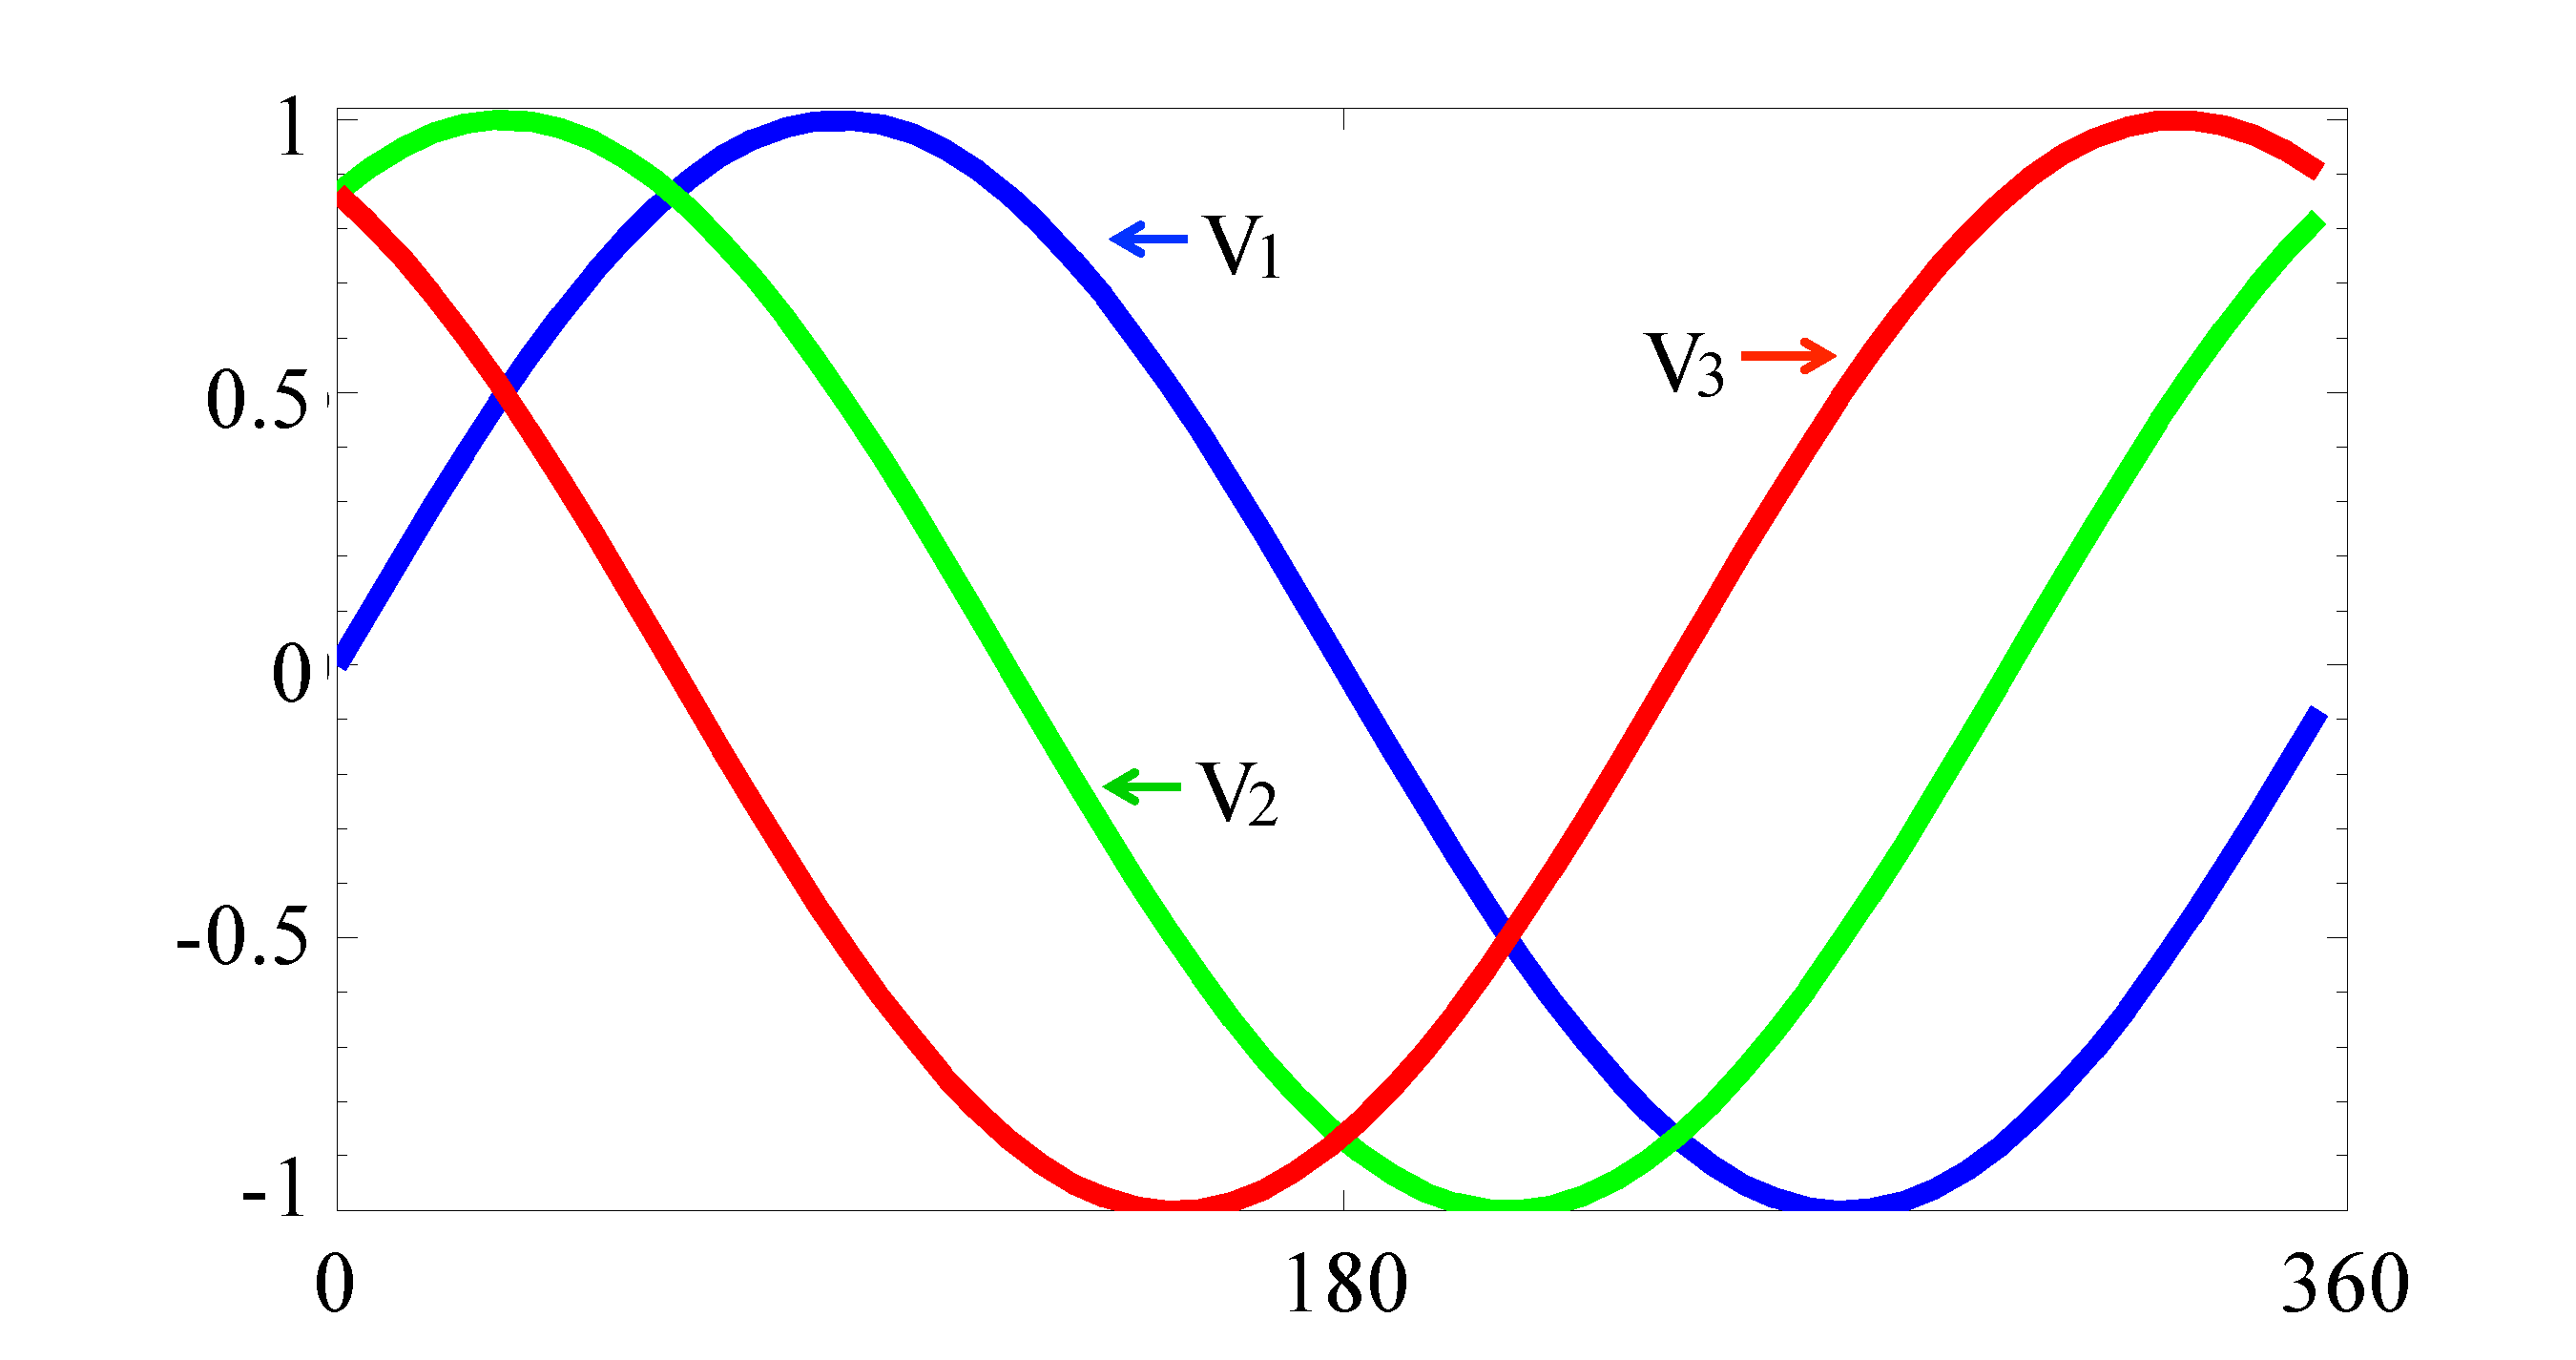
\includegraphics[width=0.4\textwidth]{figs/draw3phase.pdf}
\caption{Three phase power waveform.}
\label{fig_threephase}
\end{figure}


These three voltages can be represented mathematically
as the following three equations.
In these equations,
$\omega$ represents the frequency of
power. While the frequency varies by country, it is 50 or 60 Hz in most 
places. For example, it is 60 Hz in the U.S..

\begin{eqnarray*}
\label{eq_sinusoidal}
V_1&=& V\sin(\omega t) \\
V_2&=& V\sin(\omega t + \frac{2\pi}{3}) \\
V_3&=& V\sin(\omega t+\frac{4\pi}{3})
\end{eqnarray*}

%E can represent either voltage or current.
When a circuit is activated by a sinusoidal source voltage
with frequency $\omega$,
a current in this circuit is generated.
The relationship between current and voltage depends on
the impedance in the circuit.
Ideally, there are three types of impedance: resistor,
inductor, and capacitor.
Resistors draw power and generate heat.
An example of this is an electrical stove.
Capacitors store energy in an electrical field.
Inductors store electrical energy in a magnetic field.
Figure~\ref{fig_threebasicloads} shows three idealized AC circuits
with only resistor $R$ in the unit of ohm ($\Omega$), inductor $L$ in the unit of henry ($H$) or capacitor $C$ in the unit of faradays ($F$)
where $V_s(t)$ and current $i(t)$ are AC voltage and current.  
\begin{figure}[ht]
\centering
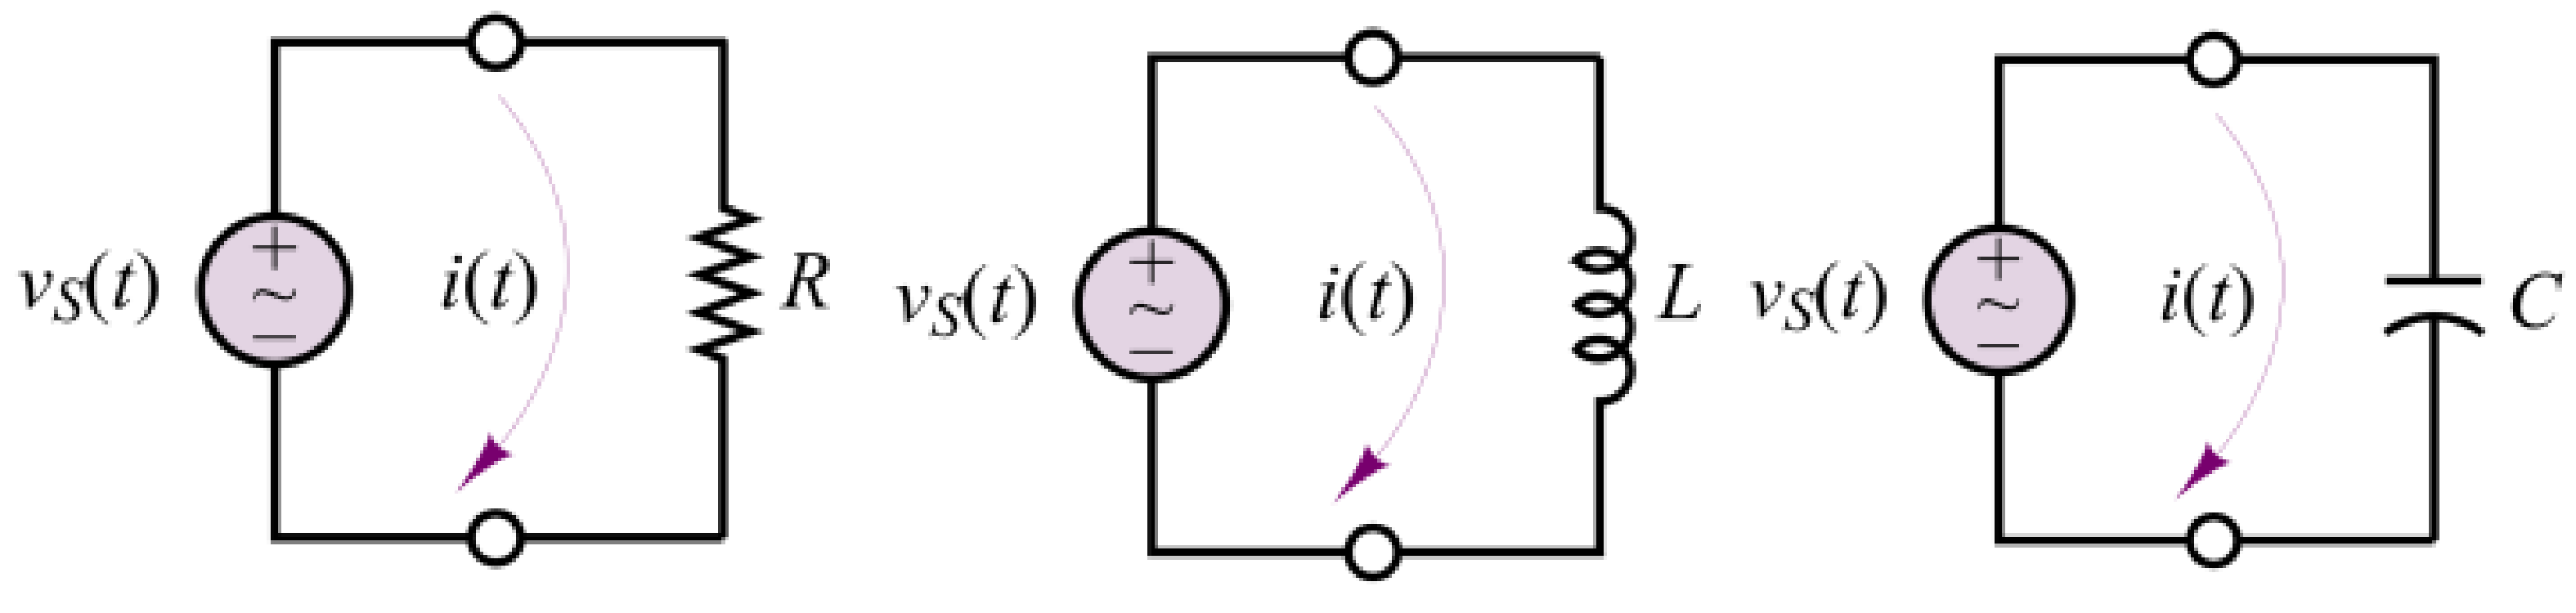
\includegraphics[width=3.3in]{figs/threebasicloads.pdf}
\caption{AC Circuit of basic loads: resistor, inductor, and capacitor (courtesy: \cite{eebook}).}
\label{fig_threebasicloads}
\end{figure}


The $i$-$v$ relationship for each circuit element of these
three types of impedance is described by the following formulas.
For the resistor circuit, according to Ohm's law $V=I R$,
\begin{equation}
i_R(t)=\frac{V_s(t)}{R}=\frac{A}{R}cos(\omega t).
\end{equation}
%The representative of R in Figure\ref{fig_simplecircuit}
%can be replaced by other loads.
For the inductor circuit, the relationship between current and voltage is
\begin{equation}
i_L(t)=\frac{A}{\omega L}cos(\omega t- \frac {\pi}{2})
\end{equation}
For the capacitor circuit, the relationship between current and voltage is
\begin{equation}
i_C(t)= \omega CAcos(\omega t + \frac {\pi}{2})
\end{equation}
where $A$ represents the amplitude, 
and $\omega$ denotes the frequency.

%\manishc{some of the symbols are not defined here. also, you use E for voltage
%  in the previous equations, and use V here.}
%\huijuanc{the symbols are explained in the above paragraph. The voltage symbol is unified as V.}  
In practice the impedance of any electrical device is composed of
at least one of these three types: 
resistors, inductor, and capacitor.
A device may include several resistor units or
inductor units or capacitor units.
For example, the mainboard of a computer 
typically contains a number of capacitors.

%%%%%%%%%%%%%%%%
\subsection{Real Power and Reactive Power}
\label{sec_pvCalculation}
In the field of electrical engineering,
real power and reactive power are concepts used
to characterize the power consumption of electric devices.
Meters typically measure current in amperes (A),
voltage in volts (V),
real power in watts (W) and
reactive power in volt-ampere reactive (VAR).

A scatter plot of real power and reactive power for different devices
is given in 
Figure~\ref{fig_realReactive_hart1992}.
The water heater, IR light, and fan only consume
real power (no reactive power) because
these devices are composed exclusively of resistors.
The values of real power of these three devices
are different from each other.
The refrigerator and water pump have similar reactive
power at around 450 VARs, but their
real power values are 750 W and 250 W, respectively.
\begin{figure}[ht]
\centering
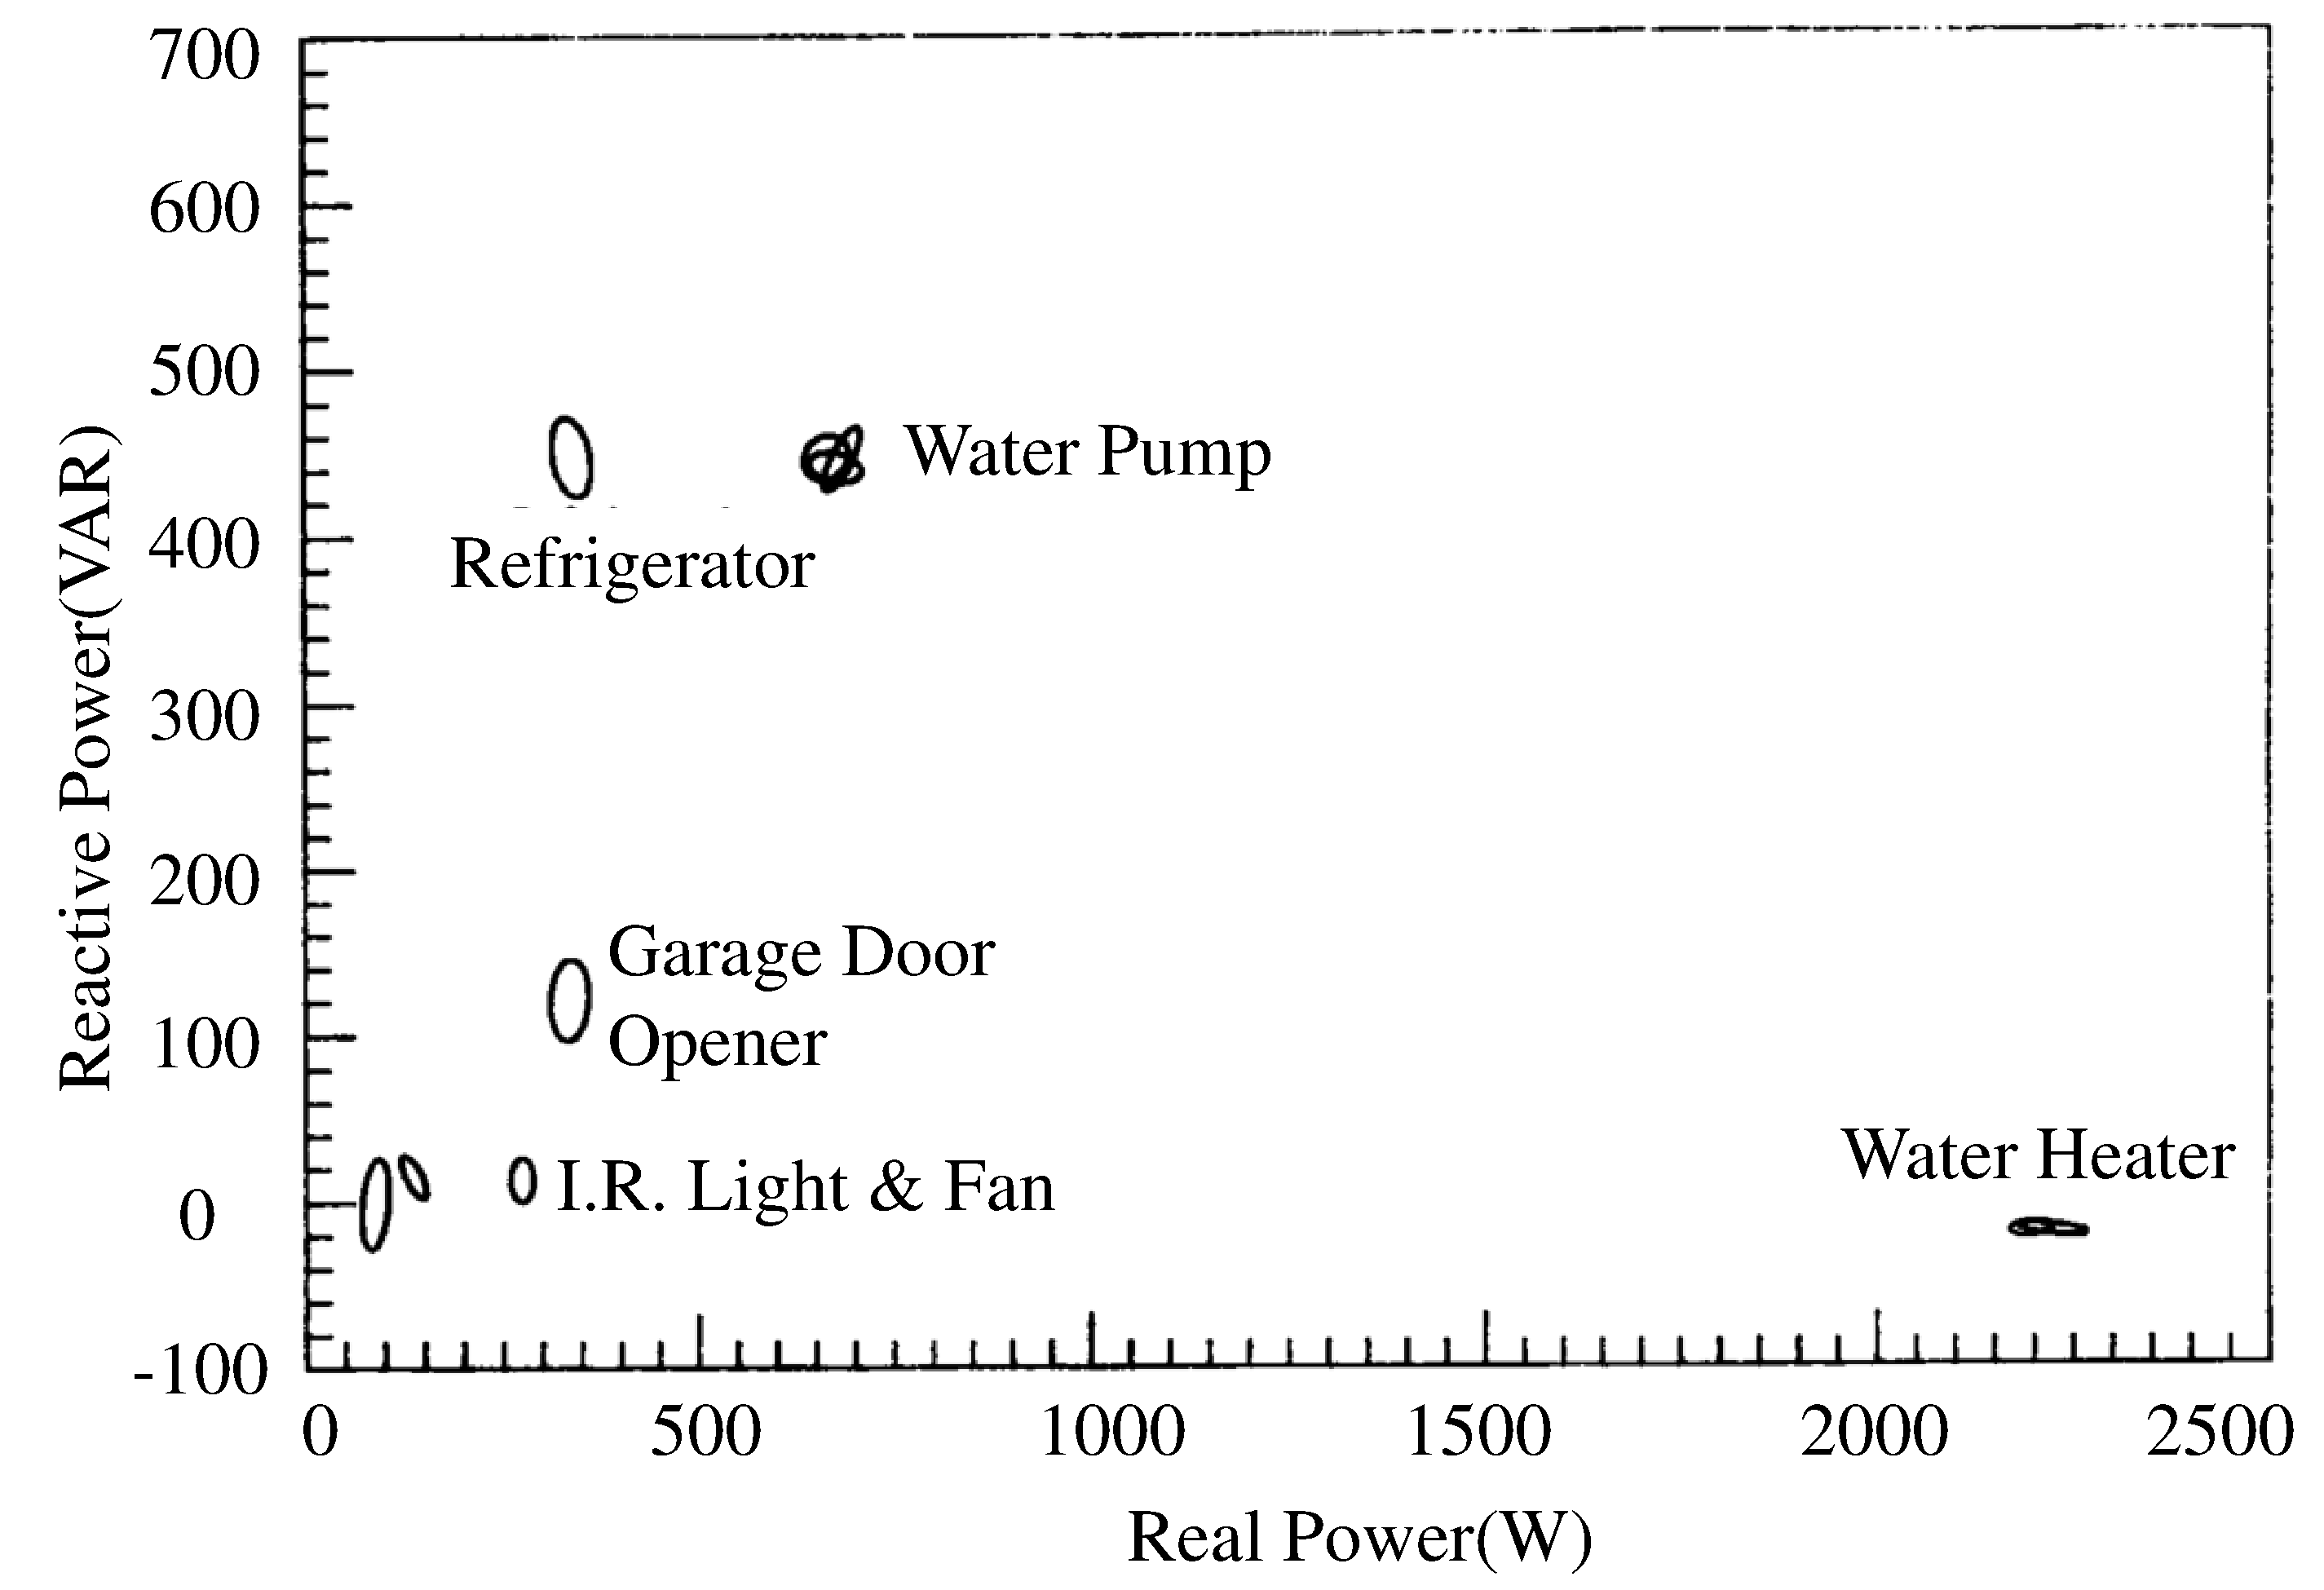
\includegraphics[width=4in]{figs/realReactive_hart1992.pdf}
\caption{Real and reactive power for different devices (courtesy: \cite{hart1992}).}
\label{fig_realReactive_hart1992}
\end{figure}


Real power and reactive power values can be
obtained by the values of voltage, current, frequency of AC power and the phase angles of voltage and current. 
Suppose we have voltage, $v(t)= V cos(\omega t - \theta_V)$ and current, $i(t)= I cos(\omega t - \theta_I)$,
%\begin{eqnarray*}
%\label{eq_voltageCurrent}
%v(t)= V cos(\omega t - \theta_V) \\
%i(t)= I cos(\omega t - \theta_I)
%\end{eqnarray*}
where $\omega$ is the base frequency of AC power,
$\theta_V$ denotes the phase angle of voltage and
$\theta_I$ represents the phase angle of current.

Instantaneous real power at time $t$ is given by:
\begin{equation}
\label{eq_insPower}
P(t)= v(t) \cdot i(t)
\end{equation}
The average root mean squared (RMS) real power usage over a period of time is typically what is
used to measure power consumption in our electricity bill.
Assume $V$ and $I$ represent the maximal value of voltage and current, then
$V_{rms} = \tilde{V} = \frac{V}{\sqrt{2}}$ and $I_{rms} = \tilde{I} = \frac{I}{\sqrt{2}}$.
The average power $P_{av}$ is the inner product of voltage and current $P_{av}=\tilde{V}\tilde{I}cos\theta$, 
where $\theta$ is the phase difference between voltage and current,
i.e. $\theta= \theta_V - \theta_I$.

%It is calculated as Equation.\ref{eq_rmsPower}.
%\begin{subequations}
%\begin{align}
%V_{rms}&=& \frac{V}{\sqrt{2}} \\%= \tilde{V} \\
%I_{rms}&=& \frac{I}{\sqrt{2}} \\%= \tilde{I} \\
%P_{av} &=& \tilde{V}\tilde{I}cos\theta \label{eq_rmsPower}
%\end{align}
%\end{subequations}
%where .
%$P_{av}$ is the average power generated by voltage and current.

%$\tilde{V}$ and $\tilde{I}$ are the RMS value of voltage and current.

The relationship between real power and reactive power is summarized in
Figure~\ref{fig_powerTriangle} and by
Equation (\ref{eq_powerTriangle}).
\begin{subequations}
\begin{align}
S=\tilde{V}\tilde{I}cos\theta+ j\tilde{V}\tilde{I}sin\theta \\
S=P_{av}+j Q \label{eq_powerTriangle}
\end{align}
\end{subequations}
\noindent
where $S$ is the apparent power,
$P$ is the average real power,
and $Q$ is the reactive power.

\begin{figure}[ht]
\centering
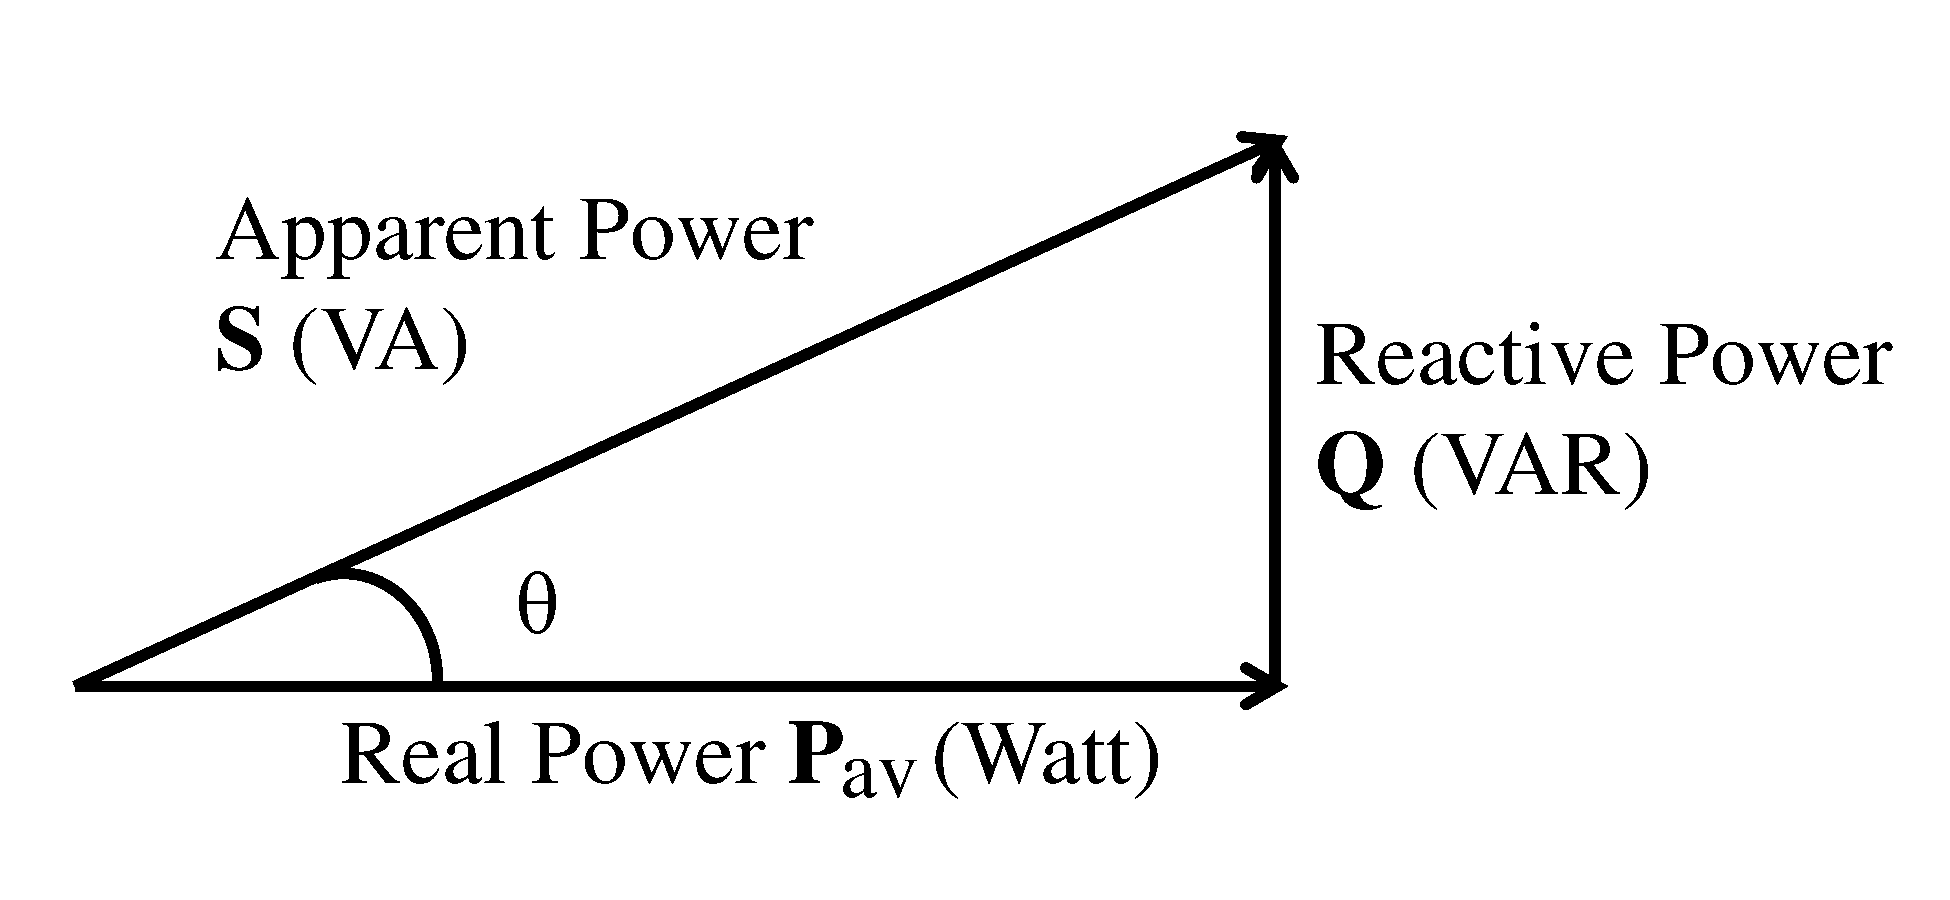
\includegraphics[width=1.8in]{figs/powerTriangle.pdf}
\caption{Power Triangle.}
\label{fig_powerTriangle}
\end{figure}


From Figure~\ref{fig_powerTriangle},
we can calculate the power factor, $\cos\theta$.
For resistive devices, the power factor is equal to 1,
which means there is only real power consumed when the device is on. 
For pure inductive or capacitive devices, the power factor equals 0,
which means there is only reactive power consumed when the device is on.
If a device has resistor $R$ $ohms$, inductor $X_L$ $henries$, and capacitor $X_C$ $farads$,
then the real power and reactive power values are
as given by 
Equations (\ref{eq_devicePowerValue}) and (\ref{eq_devicePowerValue1}).
\begin{subequations}
\begin{align}
\label{eq_devicePowerValue}
P_{av}=R\cdot I^2 \\
Q=(X_L - X_C)\cdot I^2 \label{eq_devicePowerValue1}
\end{align}
\end{subequations}

\subsection{Harmonics}
For those circuits containing an inductor or capacitor,
the current waveform is typically non-sinusoidal as shown in
Figure~\ref{fig_harmonicsexample} (a), an example taken from
the current waveform of a cycle of Circuit4 in the BLUED dataset
described later in the survey~\cite{anderson2012blued}. 
%%%\include{harmonicsexample.tex}
%\begin{figure}[ht]
%\centering
%\includegraphics[width=3.2in]{figs/harmonicsexample.pdf}
%\caption{Harmonics (courtesy: \cite{eebook}).}
%\label{fig_harmonicsexample}
%\end{figure}
\begin{figure*}[h]
	\centering{
    \begin{tabular}{cc}	
	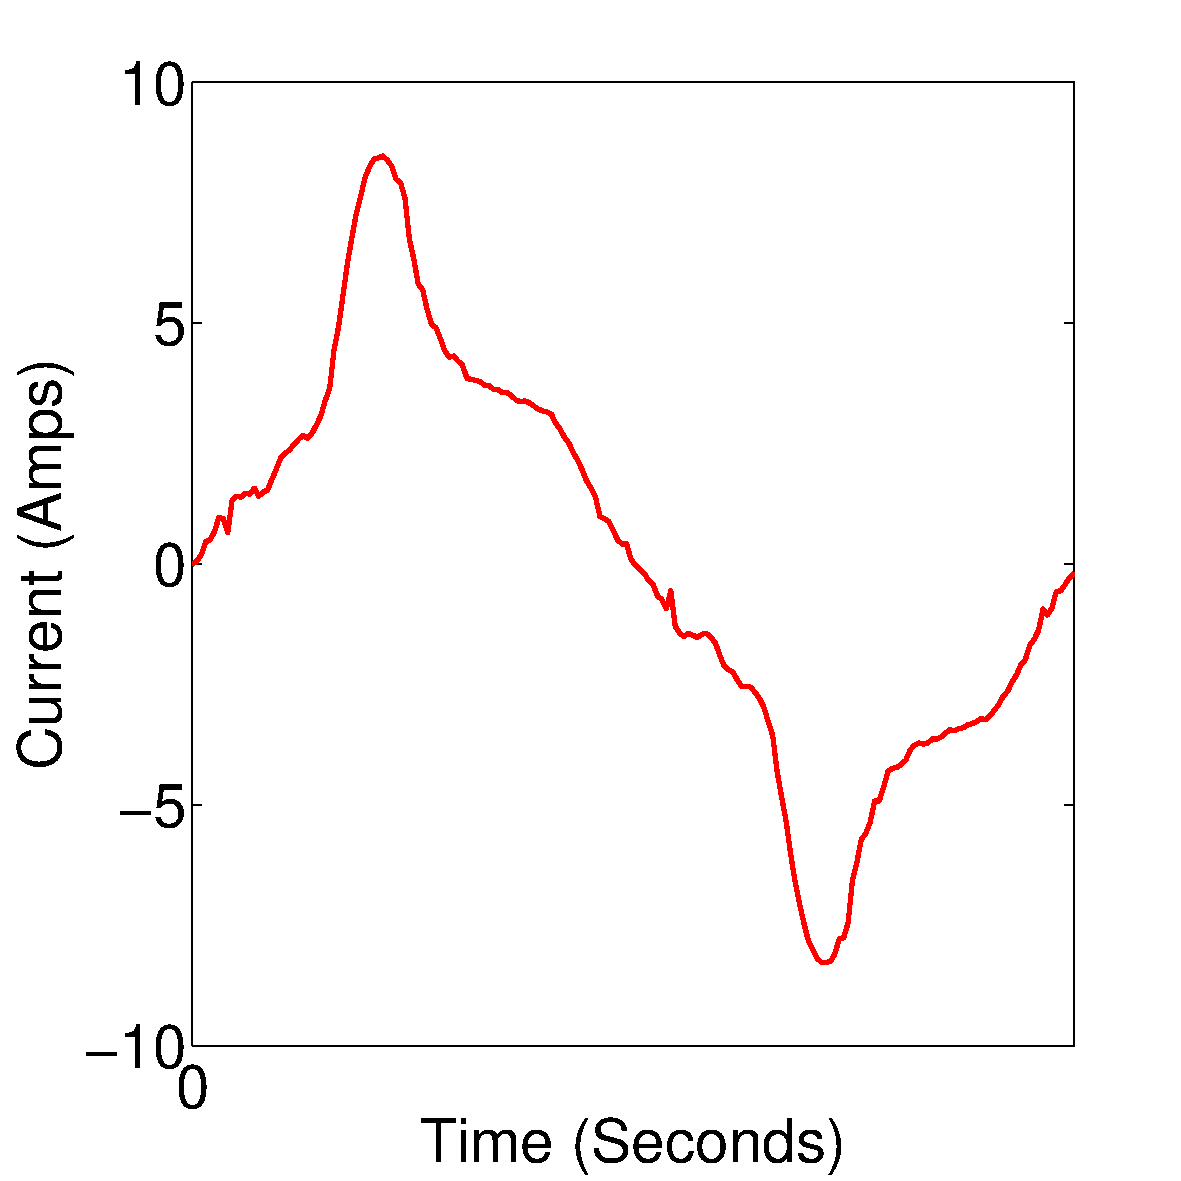
\includegraphics[width=0.4\textwidth,height=0.3\textheight]{figs/Circuit4TransientSingle.pdf} \hspace{1em}&
    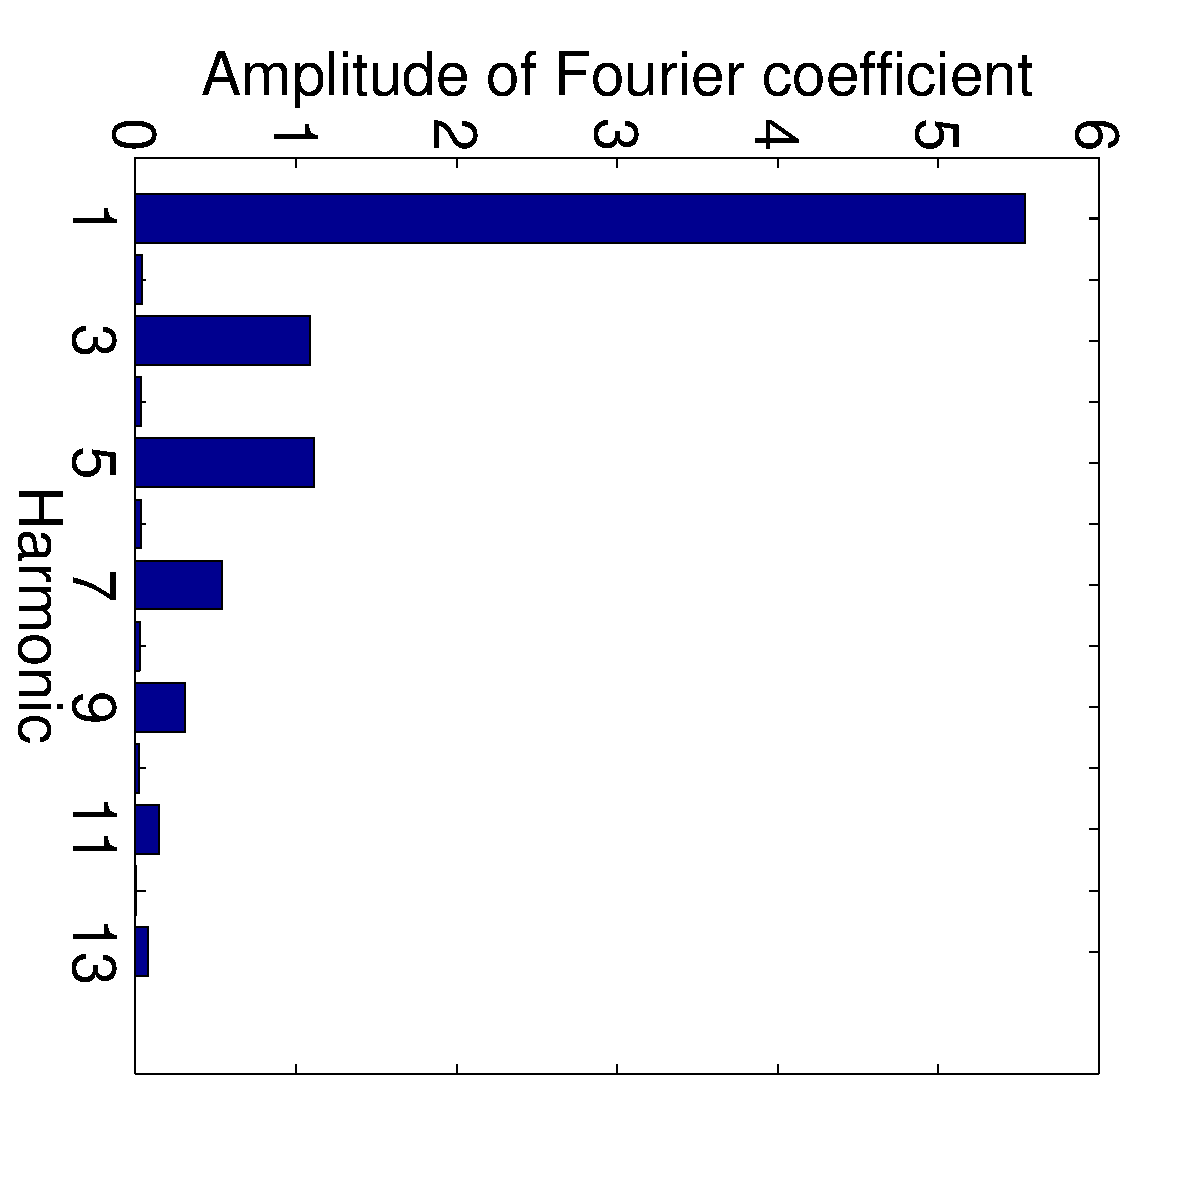
\includegraphics[width=0.4\textwidth,height=0.3\textheight,angle=90]{figs/circuit4TransientFFT.pdf} \tabularnewline
    (a) & (b)\tabularnewline
    \end{tabular}
    }
	\caption{Circuit 4 (a) Current Waveform and (b) Harmonics.}
	\label{fig_harmonicsexample}
\end{figure*}

%\begin{figure}[ht]
%\centering
%\includegraphics[width=3.2in]{figs/harmonicsexample.pdf}
%\caption{Harmonics (courtesy: \cite{eebook}).}
%\label{fig_harmonicsexample}
%\end{figure}
\begin{figure*}[h]
	\centering{
    \begin{tabular}{cc}	
	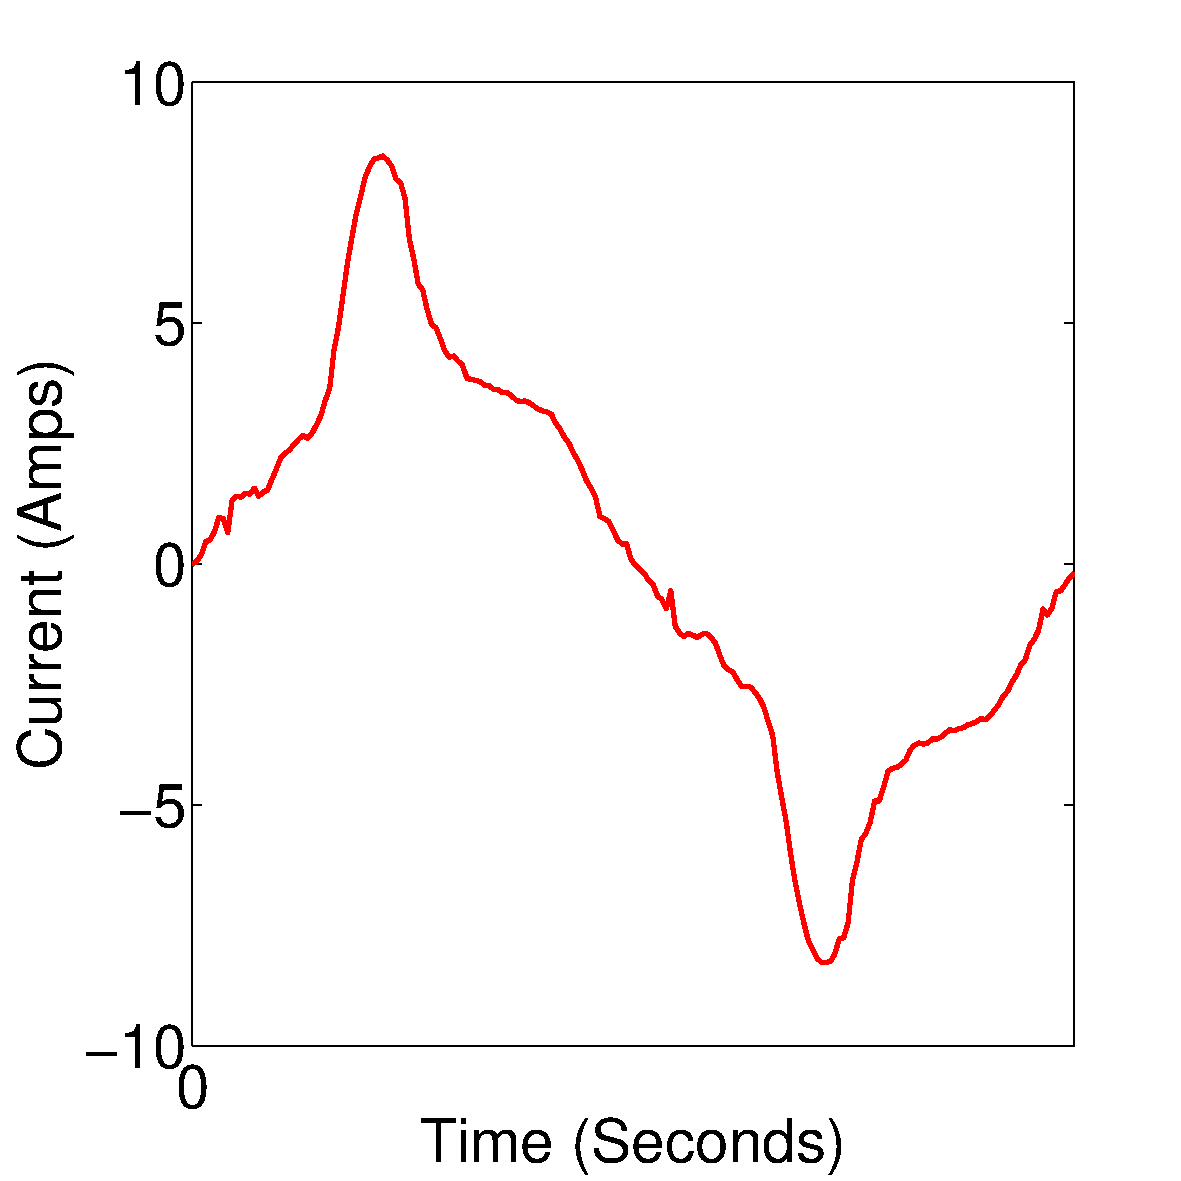
\includegraphics[width=0.4\textwidth,height=0.3\textheight]{figs/Circuit4TransientSingle.pdf} \hspace{1em}&
    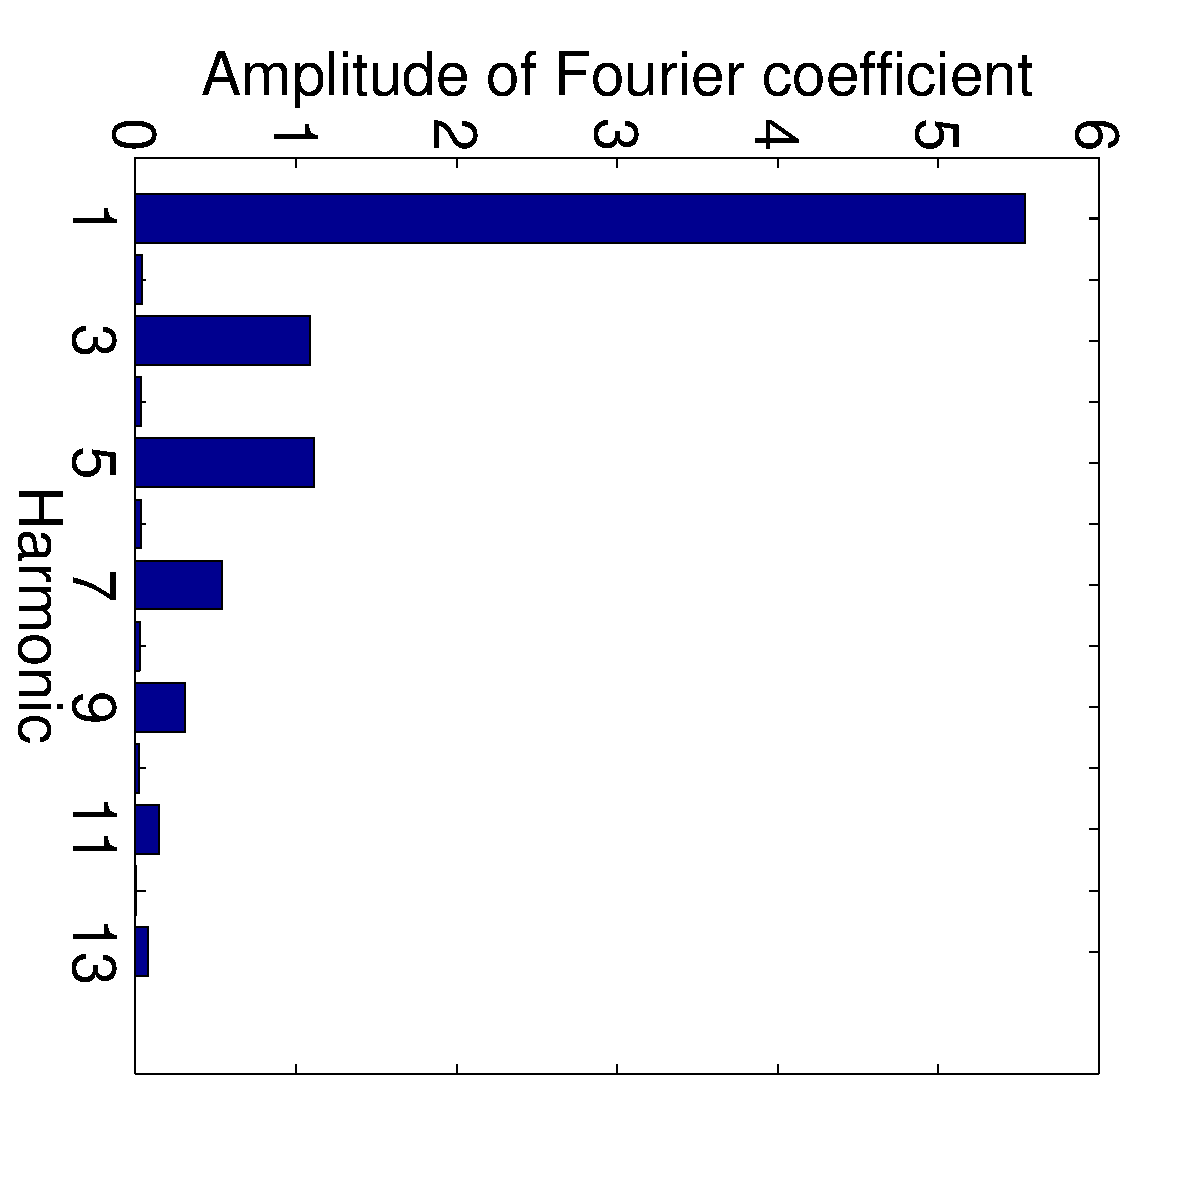
\includegraphics[width=0.4\textwidth,height=0.3\textheight,angle=90]{figs/circuit4TransientFFT.pdf} \tabularnewline
    (a) & (b)\tabularnewline
    \end{tabular}
    }
	\caption{Circuit 4 (a) Current Waveform and (b) Harmonics.}
	\label{fig_harmonicsexample}
\end{figure*}

%\begin{figure}[ht]
%\centering
%\includegraphics[width=3.2in]{figs/harmonicsexample.pdf}
%\caption{Harmonics (courtesy: \cite{eebook}).}
%\label{fig_harmonicsexample}
%\end{figure}
\begin{figure*}[h]
	\centering{
    \begin{tabular}{cc}	
	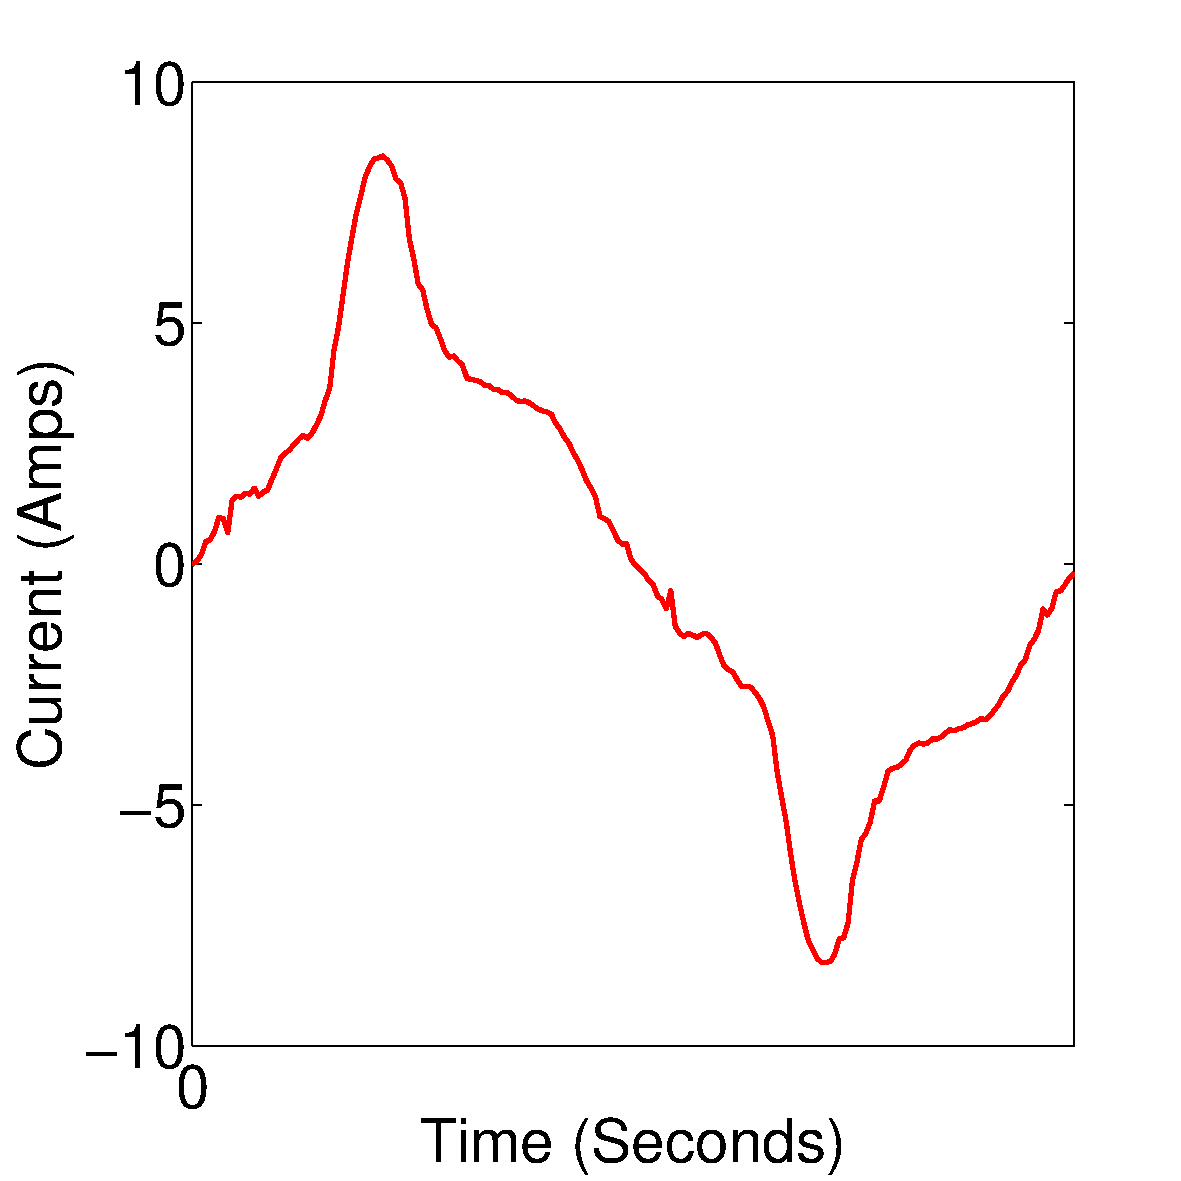
\includegraphics[width=0.4\textwidth,height=0.3\textheight]{figs/Circuit4TransientSingle.pdf} \hspace{1em}&
    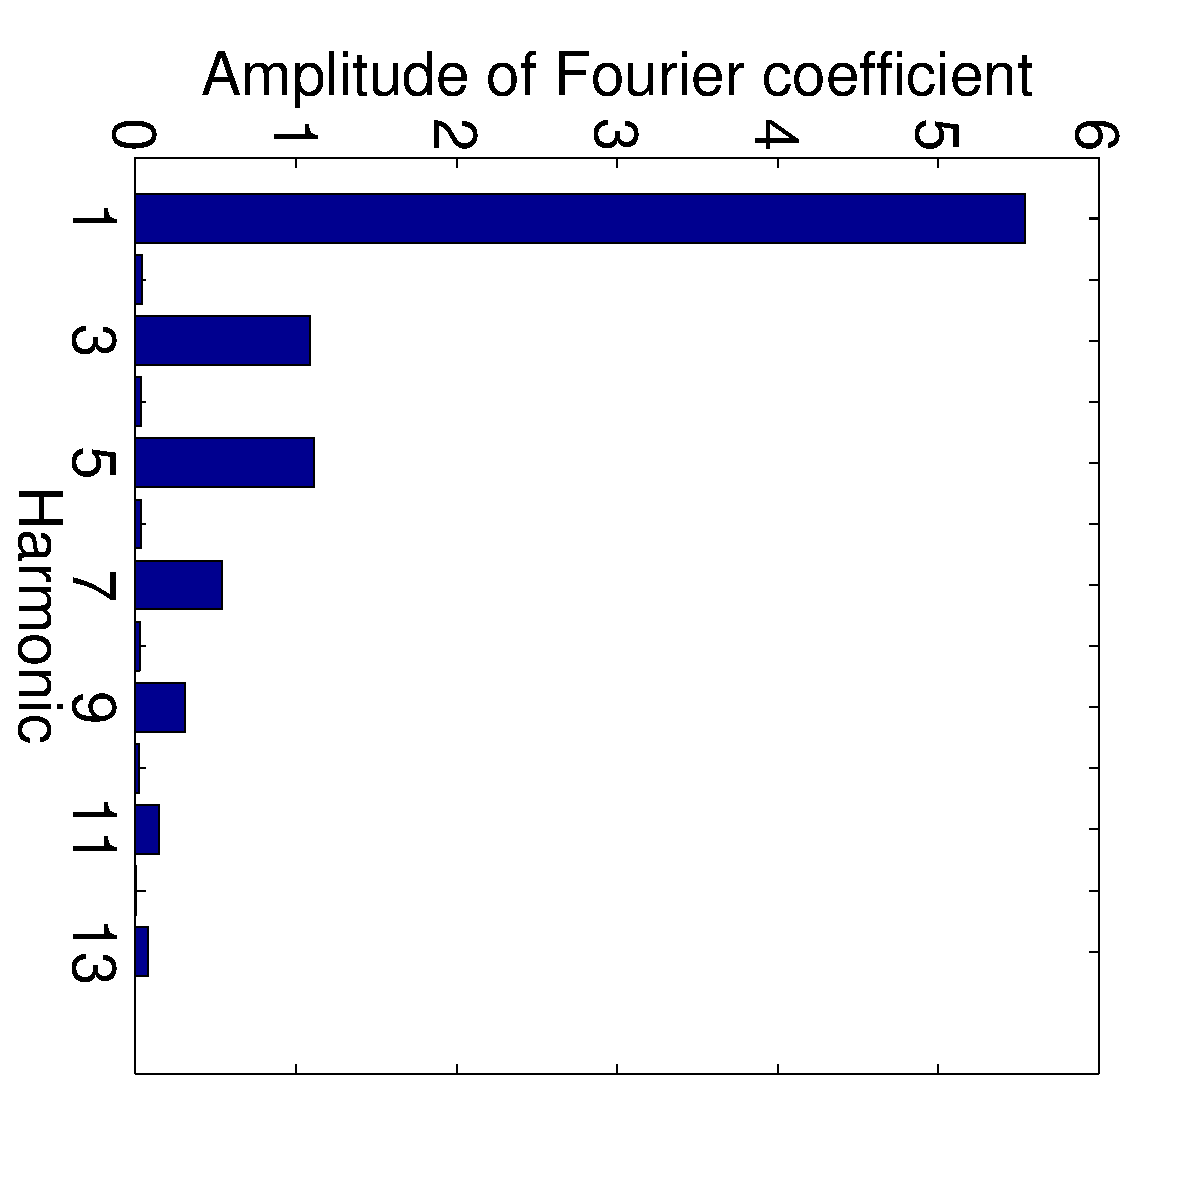
\includegraphics[width=0.4\textwidth,height=0.3\textheight,angle=90]{figs/circuit4TransientFFT.pdf} \tabularnewline
    (a) & (b)\tabularnewline
    \end{tabular}
    }
	\caption{Circuit 4 (a) Current Waveform and (b) Harmonics.}
	\label{fig_harmonicsexample}
\end{figure*}

This (or any) type of waveform can be expressed as a Fourier series.
Consider a periodic waveform $x(t) = x(t+T_0)$,
%\begin{equation}
%\label{eq_fourier}
%x(t) = x(t+T_0)
%\end{equation}
where $T_0$ is the period.
$x(t)$ can be
rewritten as
\begin{equation}
x(t) = \sum_{n=0}^{\infty}A_n cos(\frac{2\pi nt}{T}+\theta_n)
\end{equation}
where $\omega = \frac{2\pi}{T} = 2\pi f$,
$A_n$ denote the amplitudes and $\theta_n$ denote the phases.
Here $\omega$ is the fundamental frequency;
the integer multiples of basic frequencies $2\omega$, $3\omega$,
and so on are referred to as {\it harmonics}.
Figure~\ref{fig_harmonicsexample} (b) 
depicts a Fourier spectrum of
the current waveform of Figure~\ref{fig_harmonicsexample} (a).
The x-axis is the ordered harmonics and
y-axis shows the amplitude of harmonics.
%To identify electrical harmonics,
%we usually study
%harmonics in the odd number, e.g.
Typically, odd harmonics are of interest, e.g.,
3rd harmonic, 5th harmonic, and so on.



%%%%%%%%%%%%%%%%%%%%%%%%%%%%%%%%%%%%%%%%%%%%%%%%%%%%%%%%%%%%%%%%%%

%\subsubsection{Three Typical Types of Devices}
%Generally there are three types of devices or loads,
%namely electrothermal devices, electromechanical devices
%and  power electronic devices.
%In this part, we will focus on the transient states of
%different kinds of devices.

%Electrothermal devices include incandescent lamp and
%fluorescent lamp.
%Figure\ref{fig_incadescentLamp} shows
%the transient changes of an incandescent lamp.
%The x-axis is time in unit of seconds and y-axis
%is apparent power.
%After around ten cycles, the incandescent lamp
%goes to a steady state.
%\begin{figure}[ht]
\centering
\includegraphics[width=3in]{figs/incandescentLamp.pdf}
\caption{Incandescent Lamp Transient (courtesy: \cite{leeb1993PhdThesis}).}
\label{fig_incadescentLamp}
\end{figure}


%Electromechanical loads includes direct current machines,
%induction machines
%and synchronous machines.
%The starting characteristic of motor is depicted
%in Figure\ref{fig_inductortransient}.
%The starting duration of this induction machine lasts
%for around 0.8 seconds.
%In the first 0.4 seconds, the power of this device consumes
%vibrates frequently.
%Then it goes to a relatively steady state in the second 0.4 seconds.
%\begin{figure}[ht]
%\centering
%\includegraphics[width=3in]{figs/inductortransient.pdf}
%\caption{Induction Motor Transient (courtesy: \cite{leeb1993PhdThesis}).}
%\label{fig_inductortransient}
%\end{figure}

%Electronic devices are widely used in home and office nowadays,
%such as PC, monitor, printer and so on.
%Figure\ref{fig_pctransient} depicts the generated harmonics
%when a computer starts up.
%X-axis represents time and Y-axis denotes current.
%In the first 0.12s, the harmonics changes, after that
%the PC goes to a stable state.
%\begin{figure}[ht]
%\centering
%\includegraphics[width=3in]{figs/pctransient.pdf}
%\caption{Personal Computer Transient States (courtesy: \cite{leeb1993PhdThesis}).}
%\label{fig_pctransient}
%\end{figure}

%In addition, we introduce a special device Variable Speed Devices(VSDs).
%In commercial or industrial buildings,
%VSDs are often installed to optimize the energy consumption
%and controllability.
%Now we overview the inside system of VSD to better
%understand it.
%A typical VSD is composed of a rectifier, a dc-bus link,
%an inverter and an induction motor as Figure\ref{fig_VSDsystem}
%\begin{figure}[ht]
%\centering
%\includegraphics[width=3 in]{figs/VSDsystem.png}
%\caption{Topology and typical circuit model of variable speed drive (Courtesy:\cite{lee2003PhdThesis}).}
%\label{fig_VSDsystem}
%\end{figure}
%In the front end, 60Hz alternating current inputs into the rectifier,
%in which rich harmonics are created. Then power is converted to
%DC bus then re-converted to alternating current by inverter. 

%The VSD device generate power variably instead of at a
%discrete state. For instance, it may produce power ranging from
%$100w$ to $200w$. 
%Therefore they cannot be distinguished by simply ON/OFF steady states 
%because the power changes during OFF is not the oppose value during ON.

